\clearpage
\setcounter{table}{0}
\renewcommand{\thetable}{C.\arabic{table}}
\setcounter{figure}{0}
\renewcommand{\thefigure}{C.\arabic{figure}}
\setcounter{equation}{0}
\renewcommand{\theequation}{C.\arabic{equation}}

\section{Alternative Empirical Results Using Level Readiness and Vulnerability}
\label{appendixC}

This appendix repeats the empirical exercise in Section~\ref{sec:empirical} using level ND-GAIN readiness and vulnerability measures instead of the GDP-adjusted residual-performance measures used in the main specification. The purpose is to assess whether the reduced-form spread, debt-dynamics, and single-crossing patterns are sensitive to this alternative proxy construction. The empirical workflow, sample restrictions, fixed effects, and standard-error convention are otherwise unchanged.

\subsection{Data, Proxies, and Measurement Units}

The sample is the same unbalanced non-U.S. country-year panel covering 1995--2023. The dependent variable in the spread regressions is the sovereign spread, $s_{it}$. The adaptation-readiness proxy is now
\begin{equation}
G_{it}=0.01\times readiness100_{it},
\label{eq:appc_G_def}
\end{equation}
and the vulnerability proxy is
\begin{equation}
X_{it}=0.01\times vulnerability100_{it}.
\label{eq:appc_X_def}
\end{equation}
Debt exposure remains debt/GDP, $B_{it}=0.01\times debt\_gdp_{it}$, and sovereign spreads are scaled as $s_{it}=0.01\times bond\_spreads_{it}$.

The control vector is denoted by $\mathbf{Z}_{it}=(Z_{1,it},Z_{2,it},\ldots,Z_{8,it})'$. Its components are real GDP, real GDP growth, CPI inflation, overall balance/GDP, international reserves, government effectiveness, regulatory quality, and terms of trade. All controls are scaled as in Section~\ref{sec:empirical}. Table~\ref{tab:appc_summary_stats} reports the post-preprocessing descriptive statistics under the level-proxy construction.

\begin{table}[H]\centering
\begin{threeparttable}
\caption{Post-Preprocessing Descriptive Statistics, Level-Proxies}
\label{tab:appc_summary_stats}
\scriptsize
\setlength{\tabcolsep}{2.6pt}
\begin{tabularx}{\textwidth}{llYYYYYY}
\toprule
Block & Variable & $N$ & Mean & SD & Median & Min. & Max. \\
\midrule
$S$ & Sovereign spread & 1,272 & 0.024 & 0.043 & 0.007 & -0.034 & 0.343 \\
$G$ & Readiness level & 1,798 & 0.496 & 0.143 & 0.492 & 0.179 & 0.807 \\
$B$ & Debt/GDP & 1,712 & 0.586 & 0.342 & 0.522 & 0.039 & 2.610 \\
$X$ & Vulnerability level & 1,798 & 0.382 & 0.078 & 0.367 & 0.251 & 0.581 \\
$Z_1$ & Real GDP & 1,791 & 0.080 & 0.029 & 0.077 & 0.019 & 0.163 \\
$Z_2$ & Real GDP growth & 1,787 & 0.034 & 0.036 & 0.035 & -0.145 & 0.246 \\
$Z_3$ & CPI inflation & 1,791 & 0.057 & 0.108 & 0.032 & -0.018 & 1.973 \\
$Z_4$ & Overall balance/GDP & 1,697 & -0.004 & 0.034 & -0.005 & -0.300 & 0.234 \\
$Z_5$ & International reserves & 1,753 & 0.055 & 0.128 & 0.018 & 0.000 & 1.527 \\
$Z_6$ & Government effectiveness & 1,550 & 0.006 & 0.009 & 0.007 & -0.013 & 0.025 \\
$Z_7$ & Regulatory quality & 1,550 & 0.006 & 0.008 & 0.007 & -0.013 & 0.023 \\
$Z_8$ & Terms of trade & 1,595 & 1.006 & 0.187 & 0.994 & 0.319 & 2.731 \\
\bottomrule
\end{tabularx}
\begin{tablenotes}[flushleft]\footnotesize
\item Notes: Statistics use the post-preprocessing non-U.S. 1995--2023 panel. Each row is computed on nonmissing observations for the corresponding scaled variable.
\end{tablenotes}
\end{threeparttable}
\end{table}

\subsection{Adaptation and Sovereign Financing Costs}

The baseline spread regression is identical to equation~\eqref{eq:emp_baseline_spread}, except that $G_{it}$ and $X_{it}$ are the level readiness and vulnerability proxies defined in equations~\eqref{eq:appc_G_def}--\eqref{eq:appc_X_def}. Table~\ref{tab:appc_baseline_spread} shows that the readiness coefficient remains negative and statistically significant. The coefficient on public debt is positive and significant, while the level vulnerability coefficient is close to zero in the baseline fixed-effects specification.

\begin{table}[H]\centering
\begin{threeparttable}
\caption{Baseline Fixed-Effects Estimates, Level-Proxies}
\label{tab:appc_baseline_spread}
\scriptsize
\begin{tabularx}{0.78\textwidth}{lY}
\toprule
Dependent variable & 10-year sovereign spread, $s_{it}$ \\
\midrule
$G_{it}$ & -0.055*** \\
  & (-3.209) \\
$B_{it}$ & 0.045*** \\
  & (6.480) \\
$X_{it}$ & 0.005 \\
  & (0.073) \\
\midrule
Controls $\mathbf{Z}_{it}$ & Yes \\
Country FE & Yes \\
Year FE & Yes \\
Sample period & 1995--2023 \\
Countries & 60 \\
Observations & 1,120 \\
Adjusted $R^2$ & 0.901 \\
\bottomrule
\end{tabularx}
\begin{tablenotes}[flushleft]\footnotesize
\item Notes: Robust $t$-statistics are reported in parentheses. *** $p<0.01$, ** $p<0.05$, * $p<0.10$.
\end{tablenotes}
\end{threeparttable}
\end{table}

\subsection{Heterogeneous Spread Relief and the Empirical Debt-Improving Index}

The heterogeneity regressions follow the same specifications as equations~\eqref{eq:emp_full_interaction_spread}--\eqref{eq:emp_full_interaction_spread_gz}. The empirical marginal spread relief and debt-improving index remain
\begin{equation}
\widehat m^{G,F}_{it}
=
-
\frac{\partial \widehat s_{it}}{\partial G_{it}},
\qquad
\widehat\theta^F_{it}
=
B_{it}\widehat m^{G,F}_{it}.
\label{eq:appc_theta}
\end{equation}
Under the level-proxy construction, the debt interaction is negative and statistically significant. This indicates stronger spread relief from readiness at higher debt levels. The $G_{it}\times X_{it}$ interaction is small in the parsimonious full-interaction model but becomes positive and statistically significant when $G_{it}\times\mathbf{Z}_{it}$ interactions are added, so the vulnerability-level interaction should be interpreted as proxy-specific rather than as direct evidence on vulnerability-performance sorting.

\begin{table}[H]\centering
\begin{threeparttable}
\caption{Heterogeneous Spread Relief, Level-Proxies}
\label{tab:appc_heterogeneity_spread}
\scriptsize
\setlength{\tabcolsep}{3.0pt}
\begin{tabularx}{\textwidth}{lYYYY}
\toprule
Dependent variable & \multicolumn{4}{c}{10-year sovereign spread, $s_{it}$} \\
\midrule
$G_{it}$ & 0.069*** & -0.062 & 0.063 & -0.166 \\
  & (3.233) & (-0.803) & (0.815) & (-1.498) \\
$B_{it}$ & 0.196*** & 0.045*** & 0.196*** & 0.186*** \\
  & (8.760) & (6.469) & (8.749) & (8.186) \\
$X_{it}$ & 0.074 & -0.002 & 0.068 & -0.257* \\
  & (1.067) & (-0.018) & (0.560) & (-1.936) \\
$G_{it}\times B_{it}$ & -0.276*** &  & -0.276*** & -0.261*** \\
  & (-7.734) &  & (-7.734) & (-7.192) \\
$G_{it}\times X_{it}$ &  & 0.016 & 0.014 & 0.835*** \\
  &  & (0.091) & (0.074) & (3.911) \\
\midrule
Controls $\mathbf{Z}_{it}$ & Yes & Yes & Yes & Yes \\
$G_{it}\times\mathbf{Z}_{it}$ controls & No & No & No & Yes \\
Country FE & Yes & Yes & Yes & Yes \\
Year FE & Yes & Yes & Yes & Yes \\
Countries & 60 & 60 & 60 & 60 \\
Observations & 1,120 & 1,120 & 1,120 & 1,120 \\
Adjusted $R^2$ & 0.914 & 0.900 & 0.914 & 0.918 \\
\bottomrule
\end{tabularx}
\begin{tablenotes}[flushleft]\footnotesize
\item Notes: Columns 1--4 report debt heterogeneity, vulnerability-level heterogeneity, full interaction, and full interaction with $G_{it}\times\mathbf{Z}_{it}$, respectively. Robust $t$-statistics are reported in parentheses. *** $p<0.01$, ** $p<0.05$, * $p<0.10$.
\end{tablenotes}
\end{threeparttable}
\end{table}

\begin{table}[H]\centering
\begin{threeparttable}
\caption{Empirical Debt-Improving Index Descriptive Statistics, Level-Proxies}
\label{tab:appc_theta_stats}
\scriptsize
\setlength{\tabcolsep}{3.0pt}
\begin{tabularx}{0.88\textwidth}{lYYYYYY}
\toprule
Variable & $N$ & Mean & SD & Median & Min. & Max. \\
\midrule
$\widehat{\theta}^{F}_{it}$ & 1,120 & 0.070 & 0.153 & 0.028 & -0.158 & 1.235 \\
$\widehat m^{G,F}_{it}$ & 1,120 & 0.065 & 0.108 & 0.065 & -0.382 & 0.540 \\
$\partial \widehat s_{it}/\partial G_{it}$ & 1,120 & -0.065 & 0.108 & -0.065 & -0.540 & 0.382 \\
\bottomrule
\end{tabularx}
\begin{tablenotes}[flushleft]\footnotesize
\item Notes: Statistics are computed on the expanded full-interaction spread-model estimation sample. The marginal relief variable is $\widehat m^{G,F}_{it}= -\partial \widehat s_{it}/\partial G_{it}$, and the empirical debt-improving index is $\widehat\theta^F_{it}=B_{it}\widehat m^{G,F}_{it}$.
\end{tablenotes}
\end{threeparttable}
\end{table}

\subsection{Visualizing Spread Relief and the Empirical Index}

Figure~\ref{fig:appc_spread_relief} plots the marginal spread relief implied by the level-proxy full-interaction specification. Panel A varies debt/GDP while holding the vulnerability proxy at its median. Panel B varies the vulnerability proxy while holding debt/GDP at its median. The confidence intervals are delta-method intervals based on the robust variance-covariance matrix of $(\widehat{\beta}_G,\widehat{\beta}_{GB},\widehat{\beta}_{GX})$.

\begin{figure}[H]\centering
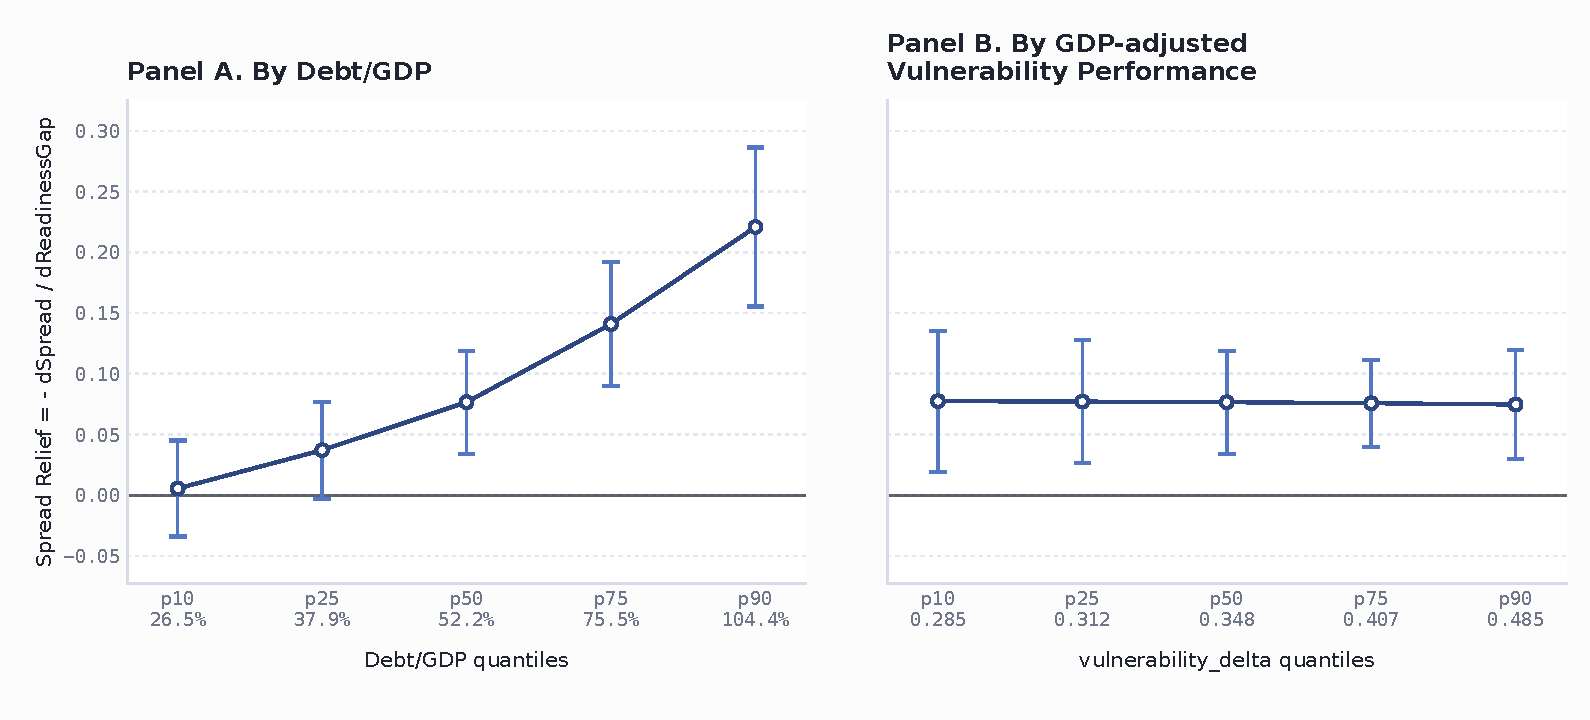
\includegraphics[width=\textwidth]{../appendixC/result/figure2.pdf}
\caption{Marginal Spread Relief from the Full-Interaction Spread Model, Level-Proxies}
\label{fig:appc_spread_relief}
\begin{minipage}{0.96\textwidth}
\footnotesize
\textit{Notes:} Panel A fixes $X_{it}$ at its median. Panel B fixes $B_{it}$ at its median. This appendix varies the level vulnerability proxy rather than the GDP-adjusted vulnerability-performance measure used in the main specification.
\end{minipage}
\end{figure}

Figure~\ref{fig:appc_theta_distribution} plots the country-year distribution of $\widehat\theta^F_{it}$ and country-level average rankings under the level-proxy construction. The dashed line marks the preferred empirical cutoff selected by the without-theta-controls kink specification.

\begin{figure}[H]\centering
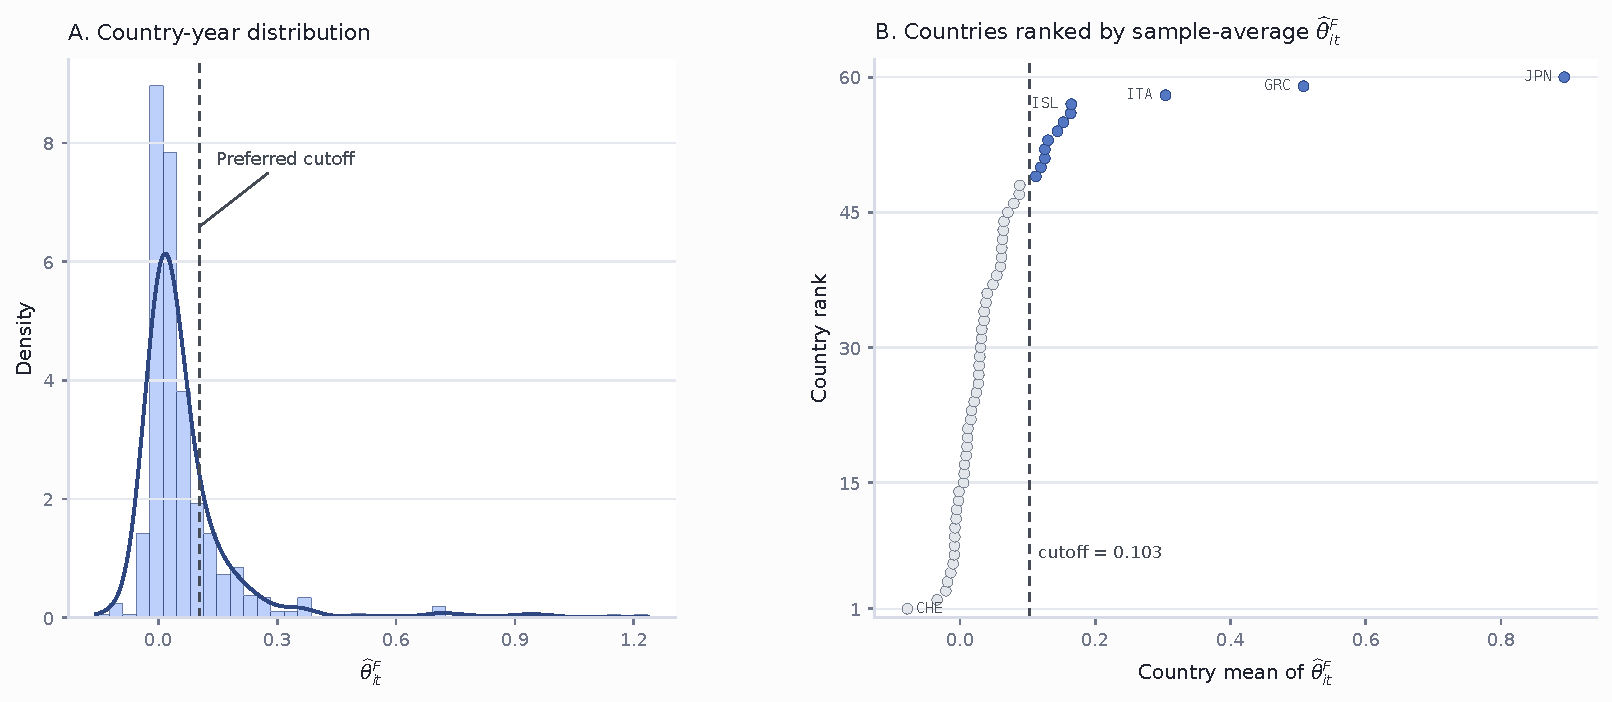
\includegraphics[width=\textwidth]{../appendixC/result/figure1_theta_distribution_cutoff.pdf}
\caption{Distribution of the Empirical Debt-Improving Index, Level-Proxies}
\label{fig:appc_theta_distribution}
\begin{minipage}{0.96\textwidth}
\footnotesize
\textit{Notes:} The left panel plots the country-year distribution of $\widehat\theta^F_{it}$. The right panel ranks countries by sample-average $\widehat\theta^F_{it}$. The dashed line marks the preferred empirical cutoff from the without-theta-controls kink specification.
\end{minipage}
\end{figure}

\subsection{Debt Dynamics and the Continuous Theta Interaction}

The debt-change regressions follow equations~\eqref{eq:emp_deltaB}--\eqref{eq:emp_debt_theta}, using the level-proxy version of $\widehat\theta^F_{it}$. Table~\ref{tab:appc_debt_change} shows that the continuous theta interaction remains negative and statistically significant. This implies that observations with higher empirical debt-improving capacity have a lower marginal effect of readiness on next-period debt changes.

\begin{table}[H]\centering
\begin{threeparttable}
\caption{Debt-Change Regressions, Level-Proxies}
\label{tab:appc_debt_change}
\scriptsize
\setlength{\tabcolsep}{3.0pt}
\begin{tabularx}{\textwidth}{lYYY}
\toprule
Dependent variable & \multicolumn{3}{c}{$\Delta B_{i,t+1}=B_{i,t+1}-B_{it}$} \\
\midrule
$G_{it}$ & -0.103*** & -0.082** & -0.090** \\
 & (-2.614) & (-2.074) & (-2.118) \\
$G_{it}\times\widehat\theta^F_{it}$ &  & -0.277*** & 0.033 \\
 &  & (-3.619) & (0.057) \\
$\widehat\theta^F_{it}$ &  &  & -0.187 \\
 &  &  & (-0.520) \\
Real GDP & 8.171*** & 4.694*** & 4.523*** \\
 & (5.412) & (3.205) & (2.914) \\
Real GDP growth & -0.326*** & -0.369*** & -0.391*** \\
 & (-3.610) & (-4.180) & (-3.854) \\
CPI inflation & -0.166** & -0.166** & -0.161** \\
 & (-1.976) & (-2.027) & (-2.095) \\
Overall balance/GDP & -0.468*** & -0.448*** & -0.436*** \\
 & (-5.849) & (-5.572) & (-5.160) \\
International reserves & 0.020 & -0.007 & -0.005 \\
 & (1.465) & (-0.475) & (-0.350) \\
Government effectiveness & -1.913** & -1.174 & -1.111 \\
 & (-2.020) & (-1.222) & (-1.134) \\
Regulatory quality & 1.921** & 0.331 & -0.029 \\
 & (2.155) & (0.358) & (-0.025) \\
Terms of trade & 0.044*** & 0.035** & 0.036** \\
 & (2.774) & (2.355) & (2.500) \\
\midrule
Theta main effect & No & No & Yes \\
Controls $\mathbf{Z}_{it}$ & Yes & Yes & Yes \\
Country FE & Yes & Yes & Yes \\
Year FE & Yes & Yes & Yes \\
Observations & 1,060 & 1,060 & 1,060 \\
Countries & 60 & 60 & 60 \\
Adjusted $R^2$ & 0.425 & 0.443 & 0.444 \\
\bottomrule
\end{tabularx}
\begin{tablenotes}[flushleft]\footnotesize
\item Notes: Columns 1--3 report the baseline model, the continuous theta interaction model, and the full-theta dynamics model, respectively. The full-theta dynamics specification includes $\widehat\theta^F_{it}$ as a direct control. Robust $t$-statistics are reported in parentheses. *** $p<0.01$, ** $p<0.05$, * $p<0.10$.
\end{tablenotes}
\end{threeparttable}
\end{table}

\subsection{Grouped Debt-Change Heterogeneity}

Table~\ref{tab:appc_grouped_debt_change} compares theta, debt-ratio, and marginal-relief sorts under the level-proxy construction. The theta and marginal-relief panels show more negative coefficients in higher groups, while the debt-ratio sort is less monotone. This is consistent with the interpretation that the composite index $B_{it}\widehat m^{G,F}_{it}$ captures more than debt exposure alone.

\begin{table}[H]\centering
\caption{Grouped Debt-Change Heterogeneity Regressions, Level-Proxies}
\label{tab:appc_grouped_debt_change}
\begin{threeparttable}
\scriptsize
\setlength{\tabcolsep}{3.0pt}
\renewcommand{\arraystretch}{1.10}
\textbf{Panel A. Full-theta groups}\\[0.45em]
\begin{tabularx}{\textwidth}{lYYYYY}
\toprule
Dependent variable & \multicolumn{5}{c}{$B_{i,t+1}-B_{it}$} \\
\cmidrule(lr){2-6}
Group & 0--20\% & 20--40\% & 40--60\% & 60--80\% & 80--100\% \\
\midrule
$G_{it}$ & 0.008 & -0.001 & -0.234*** & -0.133 & -0.417 \\
 & (0.045) & (-0.017) & (-2.803) & (-1.139) & (-1.622) \\
\midrule
Controls $\mathbf{Z}_{it}$ & Yes & Yes & Yes & Yes & Yes \\
Country FE & Yes & Yes & Yes & Yes & Yes \\
Year FE & Yes & Yes & Yes & Yes & Yes \\
Observations & 212 & 212 & 212 & 212 & 212 \\
Countries & 23 & 35 & 41 & 38 & 24 \\
Adjusted $R^2$ & 0.597 & 0.550 & 0.412 & 0.489 & 0.576 \\
\bottomrule
\end{tabularx}

\vspace{0.75em}
\textbf{Panel B. Debt-ratio groups}\\[0.45em]
\begin{tabularx}{\textwidth}{lYYYYY}
\toprule
Dependent variable & \multicolumn{5}{c}{$B_{i,t+1}-B_{it}$} \\
\cmidrule(lr){2-6}
Group & 0--20\% & 20--40\% & 40--60\% & 60--80\% & 80--100\% \\
\midrule
$G_{it}$ & 0.033 & -0.157 & -0.164** & -0.167 & -0.604** \\
 & (0.533) & (-1.169) & (-2.220) & (-1.328) & (-2.443) \\
\midrule
Controls $\mathbf{Z}_{it}$ & Yes & Yes & Yes & Yes & Yes \\
Country FE & Yes & Yes & Yes & Yes & Yes \\
Year FE & Yes & Yes & Yes & Yes & Yes \\
Observations & 212 & 212 & 212 & 212 & 212 \\
Countries & 28 & 35 & 41 & 32 & 22 \\
Adjusted $R^2$ & 0.465 & 0.482 & 0.705 & 0.397 & 0.629 \\
\bottomrule
\end{tabularx}

\vspace{0.75em}
\textbf{Panel C. Marginal-relief groups}\\[0.45em]
\begin{tabularx}{\textwidth}{lYYYYY}
\toprule
Dependent variable & \multicolumn{5}{c}{$B_{i,t+1}-B_{it}$} \\
\cmidrule(lr){2-6}
Group & 0--20\% & 20--40\% & 40--60\% & 60--80\% & 80--100\% \\
\midrule
$G_{it}$ & 0.037 & 0.045 & -0.161* & -0.316*** & -0.434 \\
 & (0.223) & (0.598) & (-1.821) & (-3.129) & (-1.426) \\
\midrule
Controls $\mathbf{Z}_{it}$ & Yes & Yes & Yes & Yes & Yes \\
Country FE & Yes & Yes & Yes & Yes & Yes \\
Year FE & Yes & Yes & Yes & Yes & Yes \\
Observations & 212 & 212 & 212 & 212 & 212 \\
Countries & 25 & 34 & 41 & 38 & 27 \\
Adjusted $R^2$ & 0.576 & 0.610 & 0.413 & 0.697 & 0.588 \\
\bottomrule
\end{tabularx}
\begin{tablenotes}[flushleft]\footnotesize
\item Notes: Each column estimates the next-period change in debt/GDP on the level readiness proxy, $G_{it}$, within the indicated subgroup. Macro control coefficients and subgroup cutoff values are omitted for compactness. Robust $t$-statistics are reported in parentheses. *** $p<0.01$, ** $p<0.05$, * $p<0.10$.
\end{tablenotes}
\end{threeparttable}
\end{table}

\subsection{Single-Crossing Kink Test}

The single-crossing specification again estimates whether the marginal effect of readiness on next-period debt changes crosses zero as a function of $\widehat\theta^F_{it}$. For a candidate cutoff $c$, the estimated without-theta-controls model is
\begin{equation}
\Delta B_{i,t+1}
=
\alpha_i+\tau_t
+aG_{it}(c-\widehat\theta^F_{it})_+
+bG_{it}(\widehat\theta^F_{it}-c)_+
+\boldsymbol{\Gamma}'\mathbf{Z}_{it}
+\varepsilon_{it}.
\label{eq:appc_kink}
\end{equation}
The implied marginal effect is
\begin{equation}
m(\theta;c)
=
a(c-\theta)_+
+
b(\theta-c)_+.
\label{eq:appc_kink_marginal}
\end{equation}

Table~\ref{tab:appc_kink_model} selects an empirical cutoff of $c=0.103037$ in the main without-theta-controls specification. Below the cutoff, the estimated marginal effect is positive; above the cutoff, it is negative. The sign pattern is therefore consistent with the single-crossing interpretation under the level-proxy construction.

\begin{table}[H]\centering
\begin{threeparttable}
\caption{Single-Crossing Kink Marginal-Effect Model, Level-Proxies}
\label{tab:appc_kink_model}
\scriptsize
\setlength{\tabcolsep}{3.0pt}
\begin{tabularx}{0.78\textwidth}{lY}
\toprule
Dependent variable & $B_{i,t+1}-B_{it}$ \\
\midrule
$G_{it}(c-\widehat\theta^F_{it})_+$ & 0.726*** \\
 & (3.667) \\
$G_{it}(\widehat\theta^F_{it}-c)_+$ & -0.225*** \\
 & (-2.890) \\
\midrule
Cutoff $c$ & 0.103 \\
RSS & 1.912 \\
Share below cutoff & 0.810 \\
Selection rule & RSS minimum; sign-consistent \\
Controls $\mathbf{Z}_{it}$ & Yes \\
Country FE & Yes \\
Year FE & Yes \\
Observations & 1,060 \\
Adjusted $R^2$ & 0.447 \\
\bottomrule
\end{tabularx}
\begin{tablenotes}[flushleft]\footnotesize
\item Notes: The exact RSS-selected cutoff is $c=0.1030368341448663$. The model includes country and year fixed effects and $\mathbf{Z}_{it}$ controls, but does not include direct theta controls. Robust $t$-statistics are reported in parentheses. *** $p<0.01$.
\end{tablenotes}
\end{threeparttable}
\end{table}

Figure~\ref{fig:appc_kink_marginal_effect} plots the continuous marginal-effect curve implied by equation~\eqref{eq:appc_kink_marginal}. The confidence band is computed by the delta method using the robust variance-covariance matrix of the two kink coefficients.

\begin{figure}[H]\centering
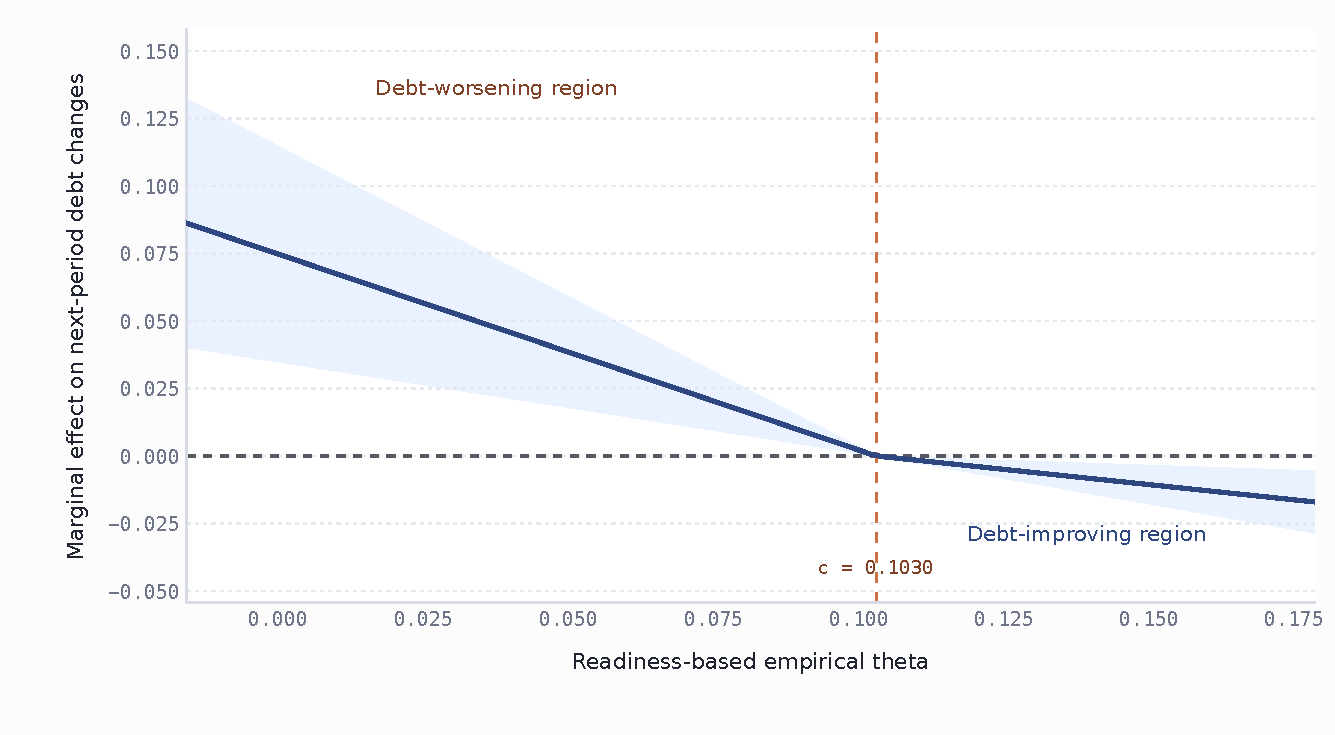
\includegraphics[width=0.92\textwidth]{../appendixC/result/figure3_kink_marginal_effect_notheta_continuous.pdf}
\caption{Continuous Kink Marginal Effect without Theta Controls, Level-Proxies}
\label{fig:appc_kink_marginal_effect}
\begin{minipage}{0.92\textwidth}
\footnotesize
\textit{Notes:} The figure plots $m(\theta;c)=a(c-\theta)_+ + b(\theta-c)_+$ from the single-crossing kink model without theta controls. Positive values imply that readiness improvements are associated with higher next-period debt changes; negative values imply lower next-period debt changes. The vertical dashed line marks the empirical cutoff $c$.
\end{minipage}
\end{figure}

\subsection{Country Screens Around the Preferred Cutoff}

Table~\ref{tab:appc_country_screens} applies the preferred cutoff to country-level screens. Under the level-proxy construction, no country satisfies the low-debt, always-above-cutoff, top-relief screening rule. Four countries satisfy the high-debt, always-below-cutoff, bottom-relief rule. As in the main text, the screen is descriptive and should not be interpreted as a structural country classification.

\begin{table}[H]\centering
\begin{threeparttable}
\caption{Country Screens Around the Preferred Cutoff, Level-Proxies}
\label{tab:appc_country_screens}
\scriptsize
\setlength{\tabcolsep}{3.0pt}
\textbf{Panel A. Low debt, theta always above the cutoff, and top-quartile marginal relief}\\[0.45em]
\begin{tabularx}{\textwidth}{llYYYYY}
\toprule
Country & ISO3 & Sample period & Years & Mean debt/GDP & Mean theta & Mean $\widehat m^{G,F}$ \\
\midrule
\multicolumn{7}{l}{No countries satisfy the screening rule.} \\
\bottomrule
\end{tabularx}

\vspace{0.75em}
\textbf{Panel B. High debt, theta always below the cutoff, and bottom-quartile marginal relief}\\[0.45em]
\begin{tabularx}{\textwidth}{llYYYYY}
\toprule
Country & ISO3 & Sample period & Years & Mean debt/GDP & Mean theta & Mean $\widehat m^{G,F}$ \\
\midrule
Croatia & HRV & 2008--2023 & 16 & 69.66\% & -0.021 & -0.034 \\
Malta & MLT & 2010--2023 & 14 & 53.91\% & -0.014 & -0.028 \\
Namibia & NAM & 2014--2023 & 10 & 53.74\% & -0.008 & -0.026 \\
Netherlands & NLD & 2000--2023 & 23 & 54.21\% & -0.007 & -0.016 \\
\bottomrule
\end{tabularx}
\begin{tablenotes}[flushleft]\footnotesize
\item Notes: The preferred cutoff is $c=0.103037$. Screening thresholds use country-level means: the mean-debt median is 53.06 percent, the bottom quartile of mean $\widehat m^{G,F}_{it}$ is 0.009, and the top quartile is 0.102. The always-above and always-below conditions are evaluated year by year.
\end{tablenotes}
\end{threeparttable}
\end{table}

\subsection{Additional Control-Set Variants}

This subsection reports the appendix control-set variants generated by the same workflow. The models parallel Appendix~\ref{appendixB}, but use the level readiness and vulnerability proxies throughout.

\begin{table}[H]\centering
\caption{Debt-Change Model Control-Set Variants, Level-Proxies}
\label{tab:appc_debt_change_control_variants}
\begin{threeparttable}
\scriptsize
\setlength{\tabcolsep}{3.0pt}
\renewcommand{\arraystretch}{1.02}
\textbf{Panel A. Baseline debt-change model}\\[0.45em]
\begin{tabularx}{\textwidth}{lYYY}
\toprule
Dependent variable & \multicolumn{3}{c}{$B_{i,t+1}-B_{it}$} \\
Control set & $\mathbf{Z}+B+X$ & $B+X$ & None \\
\midrule
$G_{it}$ & -0.066 & -0.125*** & -0.137*** \\
 & (-1.612) & (-2.898) & (-3.145) \\
$B_{it}$ & -0.085*** & -0.084*** &  \\
 & (-3.514) & (-3.951) &  \\
$X_{it}$ & 0.323 & -0.278 &  \\
 & (1.315) & (-1.276) &  \\
\midrule
Controls $\mathbf{Z}_{it}$ & Yes & No & No \\
Observations & 1,060 & 1,060 & 1,060 \\
Adjusted $R^2$ & 0.450 & 0.362 & 0.332 \\
\bottomrule
\end{tabularx}

\vspace{0.35em}
\textbf{Panel B. Continuous theta interaction model}\\[0.45em]
\begin{tabularx}{\textwidth}{lYYY}
\toprule
Dependent variable & \multicolumn{3}{c}{$B_{i,t+1}-B_{it}$} \\
Control set & $\mathbf{Z}+B+X$ & $B+X$ & None \\
\midrule
$G_{it}$ & -0.068* & -0.133*** & -0.139*** \\
 & (-1.664) & (-3.132) & (-3.289) \\
$G_{it}\times\widehat{\theta}^{F}_{it}$ & -0.100 & -0.232** & -0.332*** \\
 & (-0.905) & (-2.015) & (-4.858) \\
$B_{it}$ & -0.065* & -0.034 &  \\
 & (-1.808) & (-0.949) &  \\
$X_{it}$ & 0.343 & -0.142 &  \\
 & (1.399) & (-0.666) &  \\
\midrule
Controls $\mathbf{Z}_{it}$ & Yes & No & No \\
Observations & 1,060 & 1,060 & 1,060 \\
Adjusted $R^2$ & 0.450 & 0.369 & 0.368 \\
\bottomrule
\end{tabularx}

\vspace{0.35em}
\textbf{Panel C. Full-theta dynamics model}\\[0.45em]
\begin{tabularx}{\textwidth}{lYYY}
\toprule
Dependent variable & \multicolumn{3}{c}{$B_{i,t+1}-B_{it}$} \\
Control set & $\mathbf{Z}+B+X$ & $B+X$ & None \\
\midrule
$G_{it}$ & -0.069 & -0.141*** & -0.150*** \\
 & (-1.646) & (-2.979) & (-3.116) \\
$G_{it}\times\widehat{\theta}^{F}_{it}$ & -0.075 & -0.061 & -0.052 \\
 & (-0.131) & (-0.113) & (-0.095) \\
$\widehat{\theta}^{F}_{it}$ & -0.016 & -0.111 & -0.165 \\
 & (-0.047) & (-0.348) & (-0.507) \\
$B_{it}$ & -0.064** & -0.028 &  \\
 & (-2.199) & (-0.909) &  \\
$X_{it}$ & 0.339 & -0.160 &  \\
 & (1.260) & (-0.721) &  \\
\midrule
Controls $\mathbf{Z}_{it}$ & Yes & No & No \\
Observations & 1,060 & 1,060 & 1,060 \\
Adjusted $R^2$ & 0.450 & 0.368 & 0.368 \\
\bottomrule
\end{tabularx}
\begin{tablenotes}[flushleft]\footnotesize
\item Notes: Each specification includes country and year fixed effects. Robust $t$-statistics are reported in parentheses. *** $p<0.01$, ** $p<0.05$, * $p<0.10$.
\end{tablenotes}
\end{threeparttable}
\end{table}

For the $\mathbf{Z}_{it}+B_{it}+X_{it}$ version reported in Table~\ref{tab:appc_kink_notheta_controls}, the without-theta-controls kink specification is
\begin{equation}
\begin{aligned}
\Delta B_{i,t+1}
&=
\alpha_i+\tau_t
+aG_{it}(c-\widehat\theta^F_{it})_+
+bG_{it}(\widehat\theta^F_{it}-c)_+ \\
&\quad
+\delta_B B_{it}
+\delta_X X_{it}
+\boldsymbol{\Gamma}'\mathbf{Z}_{it}
+\varepsilon_{it}.
\end{aligned}
\label{eq:appc_kink_notheta_zbx}
\end{equation}

\begin{table}[H]\centering
\caption{Single-Crossing Kink without Theta Controls: Control-Set Variants, Level-Proxies}
\label{tab:appc_kink_notheta_controls}
\begin{threeparttable}
\scriptsize
\setlength{\tabcolsep}{3.0pt}
\begin{tabularx}{0.92\textwidth}{lYYY}
\toprule
Dependent variable & \multicolumn{3}{c}{$B_{i,t+1}-B_{it}$} \\
Control set & $\mathbf{Z}+B+X$ & $B+X$ & None \\
\midrule
$G_{it}(c-\widehat\theta^F_{it})_+$ & 1.078* & -0.202 & 0.141 \\
$p(a>0)$ & 0.050 & 0.783 & 0.240 \\
$G_{it}(\widehat\theta^F_{it}-c)_+$ & -0.118 & -0.188 & -0.339*** \\
$p(b<0)$ & 0.147 & 0.050 & 0.000 \\
\midrule
RSS cutoff & -0.002 & 0.042 & -0.016 \\
Sign-consistent & Yes & No & Yes \\
Country FE & Yes & Yes & Yes \\
Year FE & Yes & Yes & Yes \\
Observations & 1,060 & 1,060 & 1,060 \\
Adjusted $R^2$ & 0.451 & 0.366 & 0.364 \\
\bottomrule
\end{tabularx}
\begin{tablenotes}[flushleft]\footnotesize
\item Notes: These variants keep the main without-theta-controls kink structure but vary the additional controls. Reported $p$-values are one-sided tests for the sign restriction. *** $p<0.01$, * $p<0.10$.
\end{tablenotes}
\end{threeparttable}
\end{table}

For the $\mathbf{Z}_{it}+B_{it}+X_{it}$ version corresponding to Table~\ref{tab:appc_kink_withtheta_main}, the kink specification with direct theta controls is
\begin{equation}
\begin{aligned}
\Delta B_{i,t+1}
&=
\alpha_i+\tau_t
+aG_{it}(c-\widehat\theta^F_{it})_+
+bG_{it}(\widehat\theta^F_{it}-c)_+ \\
&\quad
+\rho_1\widehat\theta^F_{it}
+\rho_2(\widehat\theta^F_{it}-c)_+
+\delta_B B_{it}
+\delta_X X_{it}
+\boldsymbol{\Gamma}'\mathbf{Z}_{it}
+\varepsilon_{it}.
\end{aligned}
\label{eq:appc_kink_withtheta_zbx_main}
\end{equation}

\begin{table}[H]\centering
\begin{threeparttable}
\caption{Single-Crossing Kink with Theta Controls, Level-Proxies}
\label{tab:appc_kink_withtheta_main}
\scriptsize
\setlength{\tabcolsep}{3.0pt}
\begin{tabularx}{0.78\textwidth}{lY}
\toprule
Dependent variable & $B_{i,t+1}-B_{it}$ \\
\midrule
$G_{it}(c-\widehat\theta^F_{it})_+$ & 0.093 \\
 & (0.251) \\
$G_{it}(\widehat\theta^F_{it}-c)_+$ & 0.470 \\
 & (0.745) \\
\midrule
Direct theta controls & Yes \\
Cutoff $c$ & 0.179 \\
RSS & 1.896 \\
Share below cutoff & 0.900 \\
Selection rule & RSS minimum \\
Controls $\mathbf{Z}_{it}$ & Yes \\
Country FE & Yes \\
Year FE & Yes \\
Observations & 1,060 \\
Adjusted $R^2$ & 0.450 \\
\bottomrule
\end{tabularx}
\begin{tablenotes}[flushleft]\footnotesize
\item Notes: This appendix version includes $\widehat{\theta}^{F}_{it}$ and $(\widehat{\theta}^{F}_{it}-c)_+$ as direct controls. The with-theta-controls version does not satisfy the single-crossing sign pattern at the RSS-minimizing cutoff. Robust $t$-statistics are reported in parentheses.
\end{tablenotes}
\end{threeparttable}
\end{table}

For the $\mathbf{Z}_{it}+B_{it}+X_{it}$ column reported in Table~\ref{tab:appc_kink_withtheta_controls}, the estimated with-theta-controls variant uses the same control-augmented kink equation in \eqref{eq:appc_kink_withtheta_zbx_main}.

\begin{table}[H]\centering
\caption{Single-Crossing Kink with Theta Controls: Control-Set Variants, Level-Proxies}
\label{tab:appc_kink_withtheta_controls}
\begin{threeparttable}
\scriptsize
\setlength{\tabcolsep}{3.0pt}
\begin{tabularx}{0.92\textwidth}{lYYY}
\toprule
Dependent variable & \multicolumn{3}{c}{$B_{i,t+1}-B_{it}$} \\
Control set & $\mathbf{Z}+B+X$ & $B+X$ & None \\
\midrule
$G_{it}(c-\widehat\theta^F_{it})_+$ & 1.614** & 2.007*** & 1.495** \\
$p(a>0)$ & 0.020 & 0.004 & 0.018 \\
$G_{it}(\widehat\theta^F_{it}-c)_+$ & 0.141 & 0.234 & 0.232 \\
$p(b<0)$ & 0.593 & 0.660 & 0.656 \\
\midrule
RSS cutoff & 0.044 & 0.044 & 0.046 \\
Sign-consistent & No & No & No \\
Direct theta controls & Yes & Yes & Yes \\
Country FE & Yes & Yes & Yes \\
Year FE & Yes & Yes & Yes \\
Observations & 1,060 & 1,060 & 1,060 \\
Adjusted $R^2$ & 0.454 & 0.373 & 0.367 \\
\bottomrule
\end{tabularx}
\begin{tablenotes}[flushleft]\footnotesize
\item Notes: These variants keep direct theta controls and vary the additional controls across $\mathbf{Z}_{it}+B_{it}+X_{it}$, $B_{it}+X_{it}$, and no controls. Reported $p$-values are one-sided tests for the sign restriction. *** $p<0.01$, ** $p<0.05$.
\end{tablenotes}
\end{threeparttable}
\end{table}
